%----------------------------------------------------------------------------------------
%	PACKAGES AND OTHER DOCUMENT CONFIGURATIONS
%----------------------------------------------------------------------------------------

\documentclass[12pt]{article}

\usepackage{polski}
\usepackage[english,polish]{babel}
\usepackage[utf8]{inputenc}
\usepackage{datetime}
\usepackage{graphicx}
\usepackage{tikz}
\usepackage{amsmath}
\usepackage{multirow}
\usepackage{tabularx}
\usepackage{geometry}
\geometry{
 	a4paper, 
 	left    = 20mm,
 	right	  = 20mm,
 	top     = 20mm,
 	bottom  = 20mm,
}

\usepackage{listings}
\lstloadlanguages{TeX}

\lstset{
  literate={ą}{{\k{a}}}1
           {ć}{{\'c}}1
           {ę}{{\k{e}}}1
           {ó}{{\'o}}1
           {ń}{{\'n}}1
           {ł}{{\l{}}}1
           {ś}{{\'s}}1
           {ź}{{\'z}}1
           {ż}{{\.z}}1
           {Ą}{{\k{A}}}1
           {Ć}{{\'C}}1
           {Ę}{{\k{E}}}1
           {Ó}{{\'O}}1
           {Ń}{{\'N}}1
           {Ł}{{\L{}}}1
           {Ś}{{\'S}}1
           {Ź}{{\'Z}}1
           {Ż}{{\.Z}}1,
  basicstyle=\footnotesize\ttfamily,
}

\usepackage[
backend=biber,
style=numeric,
sorting=none,
%
% Zastosuj styl wpisu bibliograficznego właściwy językowi publikacji.
language=autobib,
autolang=other,
% Zapisuj datę dostępu do strony WWW w formacie RRRR-MM-DD.
urldate=iso8601,
% Nie dodawaj numerów stron, na których występuje cytowanie.
backref=false,
% Podawaj ISBN.
isbn=true,
% Nie podawaj URL-i, o ile nie jest to konieczne.
url=false,
%
% Ustawienia związane z polskimi normami dla bibliografii.
maxbibnames=5,
]{biblatex}

\usepackage{csquotes}
% Ponieważ `csquotes` nie posiada polskiego stylu, można skorzystać z mocno zbliżonego stylu chorwackiego.
\DeclareQuoteAlias{croatian}{polish}

\addbibresource{bibliografia.bib}
 
%----------------------------------------------------------------------------------------
 
%----------------------------------------------------------------------------------------
% DATES
%----------------------------------------------------------------------------------------

\renewcommand{\dateseparator}{.}
\newdate{exercise_date}{08}{06}{2016}

%----------------------------------------------------------------------------------------

%----------------------------------------------------------------------------------------
% TIKZ PACKAGES
%----------------------------------------------------------------------------------------

\usetikzlibrary{arrows}

%----------------------------------------------------------------------------------------

\begin{document}
 
\begin{titlepage}

\newcommand{\HRule}{\rule{\linewidth}{0.5mm}}
% Defines a new command for the horizontal lines, change thickness here

\center
% Center everything on the page
 
%----------------------------------------------------------------------------------------
%	LOGO SECTION
%----------------------------------------------------------------------------------------


\includegraphics[width=6cm]{../res/img/logo.png}\\[1cm]
% Include a department/university logo - this will require the graphicx package
 
%----------------------------------------------------------------------------------------
 
%----------------------------------------------------------------------------------------
%	HEADING SECTIONS
%----------------------------------------------------------------------------------------

\textsc{\LARGE Akademia Górniczo-Hutnicza \\[0.2cm]
im. Stanisława Staszica w Krakowie}\\[1.5cm]
% Name of your university/college

\textsc{\Large Optymalizacja w systemach sterowania}\\[0.5cm]
% Major heading such as course name

%----------------------------------------------------------------------------------------
%	TITLE SECTION
%----------------------------------------------------------------------------------------

\HRule \\[0.5cm]
{ \huge \bfseries Sterowanie czasooptymalne suwnicą}\\[0.3cm]
% Title of your document
\HRule \\[1.5cm]

\flushright
\Large \emph{Autorzy:}\\
Konrad \textsc{Adasiewcz}\\[0.1cm]  % Your name
Michał \textsc{Góra}\\[0.1cm]        % Your name
Piotr \textsc{Janus}\\[0.1cm]  % Your name
Kamil \textsc{Piszczek}\\[3cm]        % Your name
% Authors

%----------------------------------------------------------------------------------------
%	DATE SECTION
%----------------------------------------------------------------------------------------
Data wykonania sprawozdania: \\
{\large \displaydate{exercise_date}}\\[1cm]


\vfill % Fill the rest of the page with whitespace

\end{titlepage} 

\section{Wstęp}

Celem projektu była implementacja sterowania czasooptymalnego dla modelu
suwnicy, której schemat znajduje się na rysunku \ref{sch:model}.

\begin{figure}[!htb]
  \begin{center}
    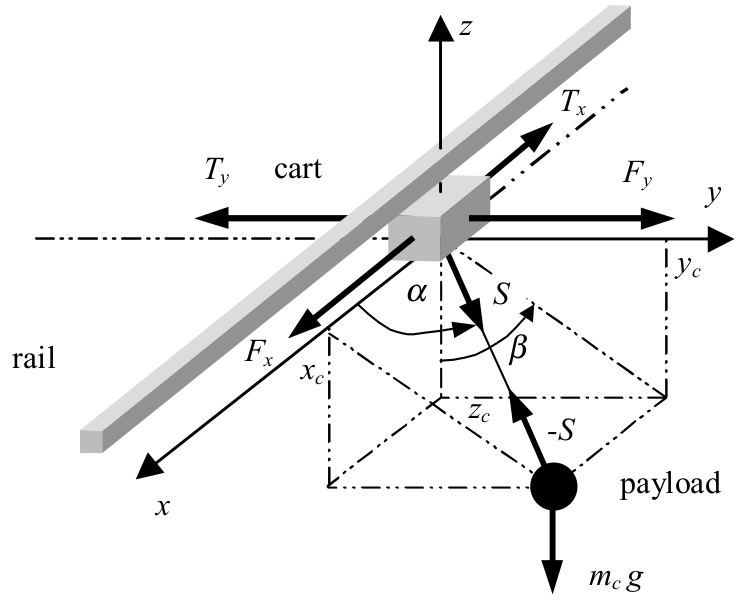
\includegraphics[width=14cm]
    {../res/img/sch-model.png}
  \end{center}
  \caption{Schemat modelu suwnicy}
  \label{sch:model}
\end{figure}

Suwnica w takiej konfiguracji, potrafi poruszać się w dwóch kierunkach w
płaszczyźnie poziomej. Ponadto długość liny nośnej jest niezależnie sterowana.
Daje to system o trzech wejściach sterujących. Taki model suwnicy można opisać
układem nieliniowych równań różniczkowych rzędu 10. Sterowanie optymalne
wyznaczone zostanie przy pomocy metody \textit{variable control
parametrization} uogólnionej na wielowejściowy system \cite{agh:vcpftop}.
Poniższa praca została w dużej części wzorowana artykułem \cite{agh:crane}.

\newpage

\section{Model matematyczny suwnicy}



\newpage

\printbibliography

\end{document}